\chapter{Data Mining in HealthCare}
\label{section:state}

Data Mining is the process of gathering knowledge from raw data. It is different from information retrieval because in that case what is
 retrieved is information that is present explicitly in the data and in the data mining case it discovers implicit patterns using analytical 
 tools. There are two types of data mining, descriptive and predictive. The former, like the name says, describes characteristics and relations
 of the existing data and the latter use the existing data to predict some future value.

Data mining has been applied in a collection of fields like CRM, finance, social networks and health care. 

One area that is becoming increasingly important is health, with the amount of data available and even the
 increase of the digitalization, to take full advantage of all this data, data mining tools need to be used. Data mining can help physicians
 to identify the most effective treatments, find adverse drug reactions, fraud detection, performing diagnostics and prognostics.

\section{Medical Diagnosis versus Prognosis}
\label{subsection:diagvsprog}

Diagnosis is the use of patient’s data, demographic and clinical, in order to under-stand and classify the current health condition of a patient.

Prognosis is the foreseeing or prediction of the risk or probability of a certain health event happening, in the future, using the clinical and
 non-clinical data. It is the medical prediction of how the pair patient disease is going to evolve in a specified period of time.

To do this prognosis, a physician will use data that relates the patient to a certain part of the population, i.e. demographic data, as well
 as the patient’s and patient’s family clinical history. This means that the evolution of the patient is important in the prediction of his next
 state. Simply putting, if a patient is showing improvement in a certain factor that is responsible for some disease, it is more probable that
 his prognosis related to that disease is better than if it the patient had the same value but that factor was deteriorating.  

As previously stated, in the process of making a prognosis a physician uses the medical history of a patient. This includes the different states 
a patient has been in the form of various clinical analysis he had done in different points over time. The need to use this sequential information 
shows the utmost importance that time has when predicting someone’s survivability, risk of recurrence.

\section{Data Mining Techniques}
\label{section:dataminingtech}

Different techniques have been used to perform all of those predictions, as we will show in the following chapter.
 We will start by describing the most common classification techniques used for prognosis, following with the cases 
 where they have been applied to perform prognosis in different diseases.

\subsection{Decision Tree}
\label{subsection:dt}

Decision trees are one of the most common classification techniques. They are a supervised learning technique that, based on the data
 features and a metric, that can be the Gini index, information gain, and Chi-squared test, tries to find the feature that best splits 
 the data into more homogeneous sets in terms of the target variable. 

By the end of the algorithm we have a tree where in each interior node there is one of the features and an edge per value of that 
feature. In the leaf nodes of this tree structure the class label is represented. An example of a decision tree is represented in Figure \ref{fig:dt}, where the outcome is whether some students will play football outside or not. If the outlook of the weather is overcast then the students will play, if it is sunny we need to look into the humidity, and if it is rainy then the wind is the deciding factor. 

\begin{figure}[!htb]
  \centering
  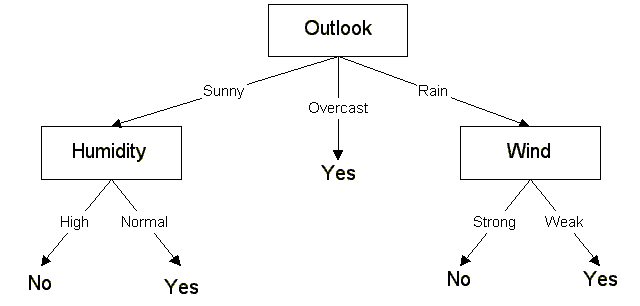
\includegraphics[width=1\textwidth]{Figures/dt.png}
  \caption{Example Decision Tree to predict if some students will play football.}
  \label{fig:dt}
\end{figure}

The most common algorithms to build decision trees are Quinlan’s ID3 \cite{Quinlan1986}, C4.5
 \cite{Quinlan1993} that came improve on ID3, and Breiman \& et al.’s Classification And 
 Regression Trees (CART) \cite{Breiman1984}.
 
 In the current work on prognosis,\hl[red]{ as seen in \ref{chapter:rw}}, the use of C5.0 is also found. C5.0 is an extension of C4.5 that, among several issues, presents a considerable performance optimization. 
 
Decision Trees result in a very easily understandable, like Figure \ref{fig:dt}, it is easy to see that some initial variable divides the data into two categories and then other variables split the resulting child groups. This information is very useful to the researcher who is trying to understand the underlying nature of the data being analyzed.

\subsection{Artificial Neural Networks \& Support Vector Machines}
\label{subsection:nn}

Artificial Neural Networks are computational models that approximate the functioning of the brain, in the sense that they are highly
 complex and non-linear. These networks are composed by a group of interconnected nodes, also called neurons, and are used for classification. 
 They have an input layer with nodes that correspond to data features, a various number of hidden layers and an output layer where the outcome 
 is represented as seen in Figure \ref{fig:nn}.

Contrarily to decision trees, neural networks do not present an easily-understandable model.
A neural network is more of a “black box” that delivers results without an explanation of how the results were derived. Thus, it is difficult or
 impossible to explain how decisions were made based on the output of the network.

\begin{figure}[!htb]
  \centering
  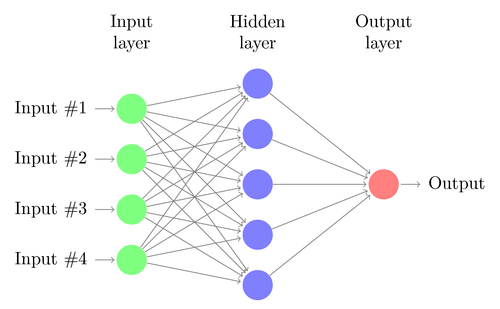
\includegraphics[width=1\textwidth]{Figures/nn.png}
  \caption{Artificial Neural Network structure.}
  \label{fig:nn}
\end{figure}

SVMs are another supervised machine learning technique, where a hyperplane is found that correctly separates the spatial representation of the data into the various classes.  For example, if the data is 2 dimensional, the hyperplane is a line that correctly divides the data and has the largest margin between itself and a data point, as seen in Figure \ref{fig:svm}. 

SVMs have been used with high accuracy and can with the right kernel can have good results even if the data is not linearly separable in the base feature space. They are memory intensive and require a lot of tunning and configuration.

 %\hl[red]{High accuracy, nice theoretical guarantees regarding overfitting, and with an appropriate kernel they can work well even if you're data isn't linearly separable in the base feature space. Especially popular in text classification problems where very high-dimensional spaces are the norm. Memory-intensive and kind of annoying to run and tune, though, so I think random forests are starting to steal the crown.}

\begin{figure}[!htb]
  \centering
  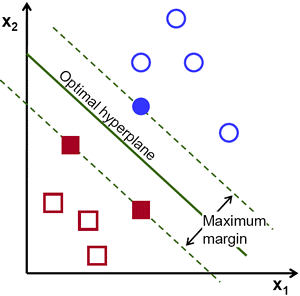
\includegraphics[width=0.75\textwidth]{Figures/svm.png}
  \caption{Example of 2D SVM optimal hyperplane.}
  \label{fig:svm}
\end{figure}

\subsection{Bayesian Classifiers}
\label{subsection:bc}

Bayesian classifiers are probabilistic classifiers that get their name by making use of the Bayes Rule of Inference. 

Naïve Bayes Classifier calculates the probability of a certain outcome class by considering that all features are independent,
 in other words by seeing how their value alone influences the outcome class. 

If the NB conditional independence assumption actually holds, a Naive Bayes classifier will converge quicker than
 discriminative models like logistic regression, so less data would be necessary.

\subsubsection{Bayesian Networks}
\label{subsubsection:bn}	

Bayesian networks are probabilistic graphical models, represented as directed acyclic graphs, where nodes represent random 
variables and edges the probabilistic dependency between them. These dependencies between variables are found using the theory of information.
% CHECK FACTS!!! \hl[red]{using statistical methods}\hl[blue]{nao +e bem assim! teoria da informaçao}. 

\hl[red]{Exemplo}

HMMs or Hidden Markov Models can be viewed as a specific case of the more general dynamic graphical models, where particular dependencies are assumed. Thus, HMMs and their variants can be interpreted as examples of DBNs.
An HMM is a stochastic finite automaton, where each state generates (emits) an observation. An HMM is described by a quintuple, ${N , M , A , B , \pi}$ where this symbols mean:

\begin{description}
	\item[$N$] = number of states in the model
	\item[$M$] = number of distinct observation symbols per state (observation symbols correspond to the physical output of the system being modelled)
	\item[$T$] = length of observation sequence
	\item[$O$] = observation sequence, i.e. , $O_1,O_2,…,O_T$
	\item[$Q$]  = state sequence $q_1,q_2,…,q_T$ in the Markov model
	\item[$A$] = ${a_{ij}}$ transition matrix, where $a_{ij}$ represents the transition probability from state $i$ to state $j$
	\item[$B$] = ${b_j (O_t)}$ observation emission matrix, where $b_j (O_t)$ represent the probability of observing $O_t$ at state $j$
	\item[$\pi$] = ${\pi_i}$ the prior probability, where $\pi_i$ represent the probability of being in state $i$ at the beginning of the
	experiment, i.e., at time $t=1$
	\item[$\lambda$] = $(A,B,\pi)$ the overall HMM model.
\end{description}

As mentioned above the HMM is characterized by $N, M, A, B$ and $\pi$. The $a_{ij}, b_i (O_t)$, and $\pi_i$ have the properties:

$ \Sigma_j a_{ij} = 1, \Sigma_t  b_i (O_t) = 1, \Sigma_i \pi_i = 1$ and  $a_{ij}, b_i (O_t)$, and $\pi_i >= 0$ for all $i,j,t$.


\subsection{Regression Analysis}
\label{subsection:regression}

Regression analysis is the use of a statistical analysis method used to measure the relation between variables. In other words, it helps to
 understand how a dependent variable varies with changes in one of the independent variables. 

Linear Regression is an example of regression analysis where a linear function is used to model the data. When the outcome variable,
 the dependent variable is binary or categorical, linear regression cannot be applied. In those cases it is used logistic regression.

 However, linear regression is appropriate only if the data can be modeled by a straight line function, which is often not 
the case.

Logistic Regression is a generalization of linear regression that, as just mentioned, is used to predict binary or categorical dependent
 variables. In this regression instead of predicting the estimate value of an event it predicts the probability of it occurring.

Regressions have comprehensible probabilistic interpretation and you can easily update your model to take in new data, unlike decision trees or SVMs. You can use this if you expect to receive more training data in the future that you want to be able to quickly incorporate into your model.

Another example of regression analysis that is also used in the healthcare domain is called Cox Proportional Hazard Models, which are a type
 of survival models, where the time to the occurrence of an event is related with one or more covariates that may be responsible. They show the 
 influence of variables in the time to an event occurrence.

In medical studies Cox Proportional hazard models are the most common method used for survival outcomes.

It is an extension of the logistic model to the survival setting. Similar to conditional logistic regression with conditioning only at time of 
events. In the logistic method we us a linear predictor while in the COX mode a hazard function is used. The hazard function dictates the risk of
 the outcome during the follow up time.
 
 \begin{equation}
  {\cal \lambda}(t|X) = {\cal \lambda}(t)e^{\beta X}
\label{eq:hazardFuntion}
\end{equation}

Where \( \lambda(t) \) is the hazard at time \(t\), and is usually estimated at the mean values of the predictors and \( \beta X\) is the linear predictor, 
\( \beta_1 \times x_1 + \beta_2 \times x_2 + ... + \beta_p \times x_p\)

 The linear predictor is usually centered at the mean value of the predictors, and \( e^\beta X \) then indicates the hazard
 ratio compared to the average risk profile.

\cleardoublepage